\documentclass[a4paper]{article}
\usepackage[T1]{fontenc}
\usepackage[utf8]{inputenc}
\usepackage[english]{babel}
% \usepackage[a4paper, total={6in, 8.5in}]{geometry}
\usepackage{amssymb}
\usepackage[hidelinks]{hyperref}
\usepackage{mathtools}
\usepackage{amsthm}
\usepackage{varioref}
\usepackage{tikz}
\usepackage{xurl}

\usetikzlibrary{positioning}

\tikzset{%
  every neuron/.style={
    circle,
    draw,
    minimum size=0.8cm
  },
  neuron missing/.style={
    draw=none, 
    scale=4,
    text height=0.2cm,
    execute at begin node=\color{black}$\vdots$
  },
}

\mathtoolsset{showonlyrefs}  

\setcounter{secnumdepth}{3}
\setcounter{tocdepth}{3}
\setlength{\parindent}{0pt}

\begin{document}
\title{Urban sound classification}
\author{Francesco Tomaselli}
\begin{titlepage}
    \begin{center}
        % \vspace*{5cm}
        \vspace*{2cm}

        \Large
        \textbf{Urban Sound classification}

        \vspace{0.5cm}
        \large
        Statistical methods for machine learning\\ experimental 
        project report
        \vspace{1.5cm}
        
        Francesco Tomaselli\\
        \small
        969853
        \vspace{.5cm}

        \vfill     
        
\includegraphics[width=.3\textwidth]{images/logo}
        \vspace*{1cm}

        \normalsize             
        University of Milan\\
        Master's Degree in Computer Science\\
        Academic year 2020/2021
             
    \end{center}
 \end{titlepage}

\tableofcontents

\vfill
\emph{I declare that this material, which I now submit for assessment, 
is entirely my own work and has not been taken from the work of others, 
save and to the extent that such work has been cited and acknowledged within 
the text of my work. I understand that plagiarism, collusion, and copying 
are grave and serious offences in the university and accept the penalties that 
would be imposed should I engage in plagiarism, collusion or copying. 
This assignment, or any part of it, has not been previously submitted by 
me or any other person for assessment on this or any other course of study.}

\setlength{\parskip}{0.7em}

\newpage

\section{Introduction}
\section{Feature extraction}
\label{feature-extraction}

This Sections presents the original dataset structure and the 
steps followed to create training and test sets from it.

Note that the models mentioned in this section are
three layers \emph{multilayer perceptron}, 
a feed forward neural network where each layer 
is densely connected  to the following, 
with a reasonable number of neurons, trained 
for 100 epochs with default parameters for the \emph{stochastic gradient 
descent optimizer}.~\cite{mlp}\cite{sgd}\\
The accuracy on the training is computed with a \emph{cross-validation} 
approach.~\cite{cross}\\
A deeper discussion about the models structure as well as the validation
techniques used in the project can be found at Section \vref{model-definition}.

\subsection{Dataset structure}
\label{dataset-structure}

The UrbanSound8k dataset contains ten folds of audio samples, each one about 
four seconds long. The samples are divided in ten classes.\\
From the total of ten folds, the number one, two, three, four and six 
are taken as a training set, the others are each one a test set.
For this reason the following count about class numerosity considers
only the five training folds.

\begin{center}
    \begin{tabular}{ |l|c| } 
        \hline
        Class name & Number of samples \\
        \hline
        air conditioner & 500 \\
        car horn & 208 \\
        children playing & 500 \\
        dog bark & 500 \\
        drilling & 500 \\
        engine idling & 517 \\
        gun shot & 190 \\
        jackhammer & 548 \\
        siren & 536 \\
        street music & 500 \\
        \hline
    \end{tabular}
\end{center}

The table shows a clear class imbalance. In particular, the classes 
\emph{car horn} and \emph{gun shot} are not as numerous as the others. 
This can lead to poor performances on the these two categories, it is
therefore taken 
into consideration with training. 

The following table shows the number of samples in the training set and 
the various test sets.

\begin{center}
    \begin{tabular}{ |l|c| } 
        \hline
        Dataset & Number of samples \\
        \hline
        Training set & 4499 \\
        Test set 5 & 936 \\
        Test set 7 & 838 \\
        Test set 8 & 806 \\
        Test set 9 & 816 \\
        Test set 10 & 837 \\
        \hline
    \end{tabular}
\end{center}
All the operations on the datasets are performed with \emph{Pandas} library.~\cite{pandas}

\subsection{First dataset}
Extracting features from audio files is not straightforward, nonetheless there 
are a collection of audio characteristics that are commonly used in audio machine learning 
applications.~\cite{features}

To extract information from audio files \emph{Librosa} is used.~\cite{librosa}
The library provides many methods to choose from,
to keep it simple, for the first try with this dataset, the extracted features 
are these three ones: 
\begin{enumerate}
    \item \emph{Mel-frequency cepstral coefficients};
    \item \emph{Chromagram};
    \item \emph{Root-mean-square}.
\end{enumerate}
Each feature consists of an array of arrays containing measurements. 
A series of functions are applied to each sub-array and results 
are concatenated in a final feature vector. 
The functions applied are \emph{minimum}, \emph{maximum}, \emph{mean} 
and \emph{median} from the \emph{Numpy} library.~\cite{numpy}

This approach results in 132 components feature vectors.

\paragraph{Parallelizing feature extraction}
Extracting the three features listed above is really intensive 
but the task is easily parallelizable, in fact, each file is independent 
from one another.

For this purpose \emph{Dask} is used to speed up the computation and 
extract features from audio files in a multi-processing fashion.~\cite{dask}
The main idea is to build an execution plan, where each audio file 
is managed in parallel by a collection of workers. 
Improvement is great as the time to process a single fold 
is cutted into a third.

\paragraph{Feature scaling}
After testing some neural networks on the first dataset results 
are not promising. One of the reasons is the big difference in 
ranges among feature vector components, for instance, 
some audio characteristics are in the order of thousands while others 
range between zero and one.

To mitigate this effect a \emph{StandardScaler} from \emph{scikit learn} is applied.~\cite{scaler}
The result is a dataset where each feature has more or less a distribution 
centered in zero with unit variance.
This leads to an improvement on the results using the same
model as before. 


\subsection{Extended dataset}
\label{extended-dataset}

Results using the three features named in the previous Subsection 
are promising but not enough, thus, to improve accuracy on the training set, 
new audio characteristics are extracted, namely:
\begin{enumerate}
    \item \emph{Zero-crossing rate};
    \item \emph{Roll-off frequency};
    \item \emph{Spectral flux onset strength}.
\end{enumerate}
As before, \emph{minimum}, \emph{maximum}, \emph{mean} 
and \emph{median} are applied to each feature vector and 
results are concatenated, leading to 12 new features for each 
audio file.
Scaling yields to promising results on the first dataset, 
so the same approach is applied to the extended one.

After testing a network on the new training set 
we can see a better accuracy.

\paragraph{Feature selection}
Adding new features can lead to better results 
in the end but they all need to be useful to the model.
For this reason the extended dataset is subject of some experiments 
with feature selection, in particular \emph{PCA} algorithm from scikit
learn is applied.~\cite{pca}

The main idea is to select a reduced number of features from the total, 
loosing as little information as possible. This approach often leads to better results, 
as useless features are discarded.

After some experiments with the number of features to select, 120 out of 144
are selected. In this case PCA application leads to a small improvement
on the training set in terms of accuracy.

\newpage
\section{Model definition}
\label{model-definition}
This Section starts by presenting how the networks used on the training set are 
structured. The second Subsection gives a detailed overview of the performances 
on the different training sets, lastly, the hyperparameter tuning phase
is described.

\subsection{Neural network structure}
The starting point for the neural network structure is a 
reasonable network in terms of hidden neurons to prevent over-fitting, 
indeed a high number of units in the hidden layers would end up in learning 
too much from the dataset, leading to poor performances on the test sets.

For this reason, the rule of thumb followed to decide hidden neurons quantity is the 
following: 
$$\#\mathit{hidden\; neurons} = \frac{2}{3}\#\mathit{input\;neurons}
+ \#\mathit{output\;neurons}$$
The next step is to decide the hidden layers number. As using the rule 
presented above gives a quite small amount of units, only two layers are considered,  
indeed, an higher quantity would mean having a real small number of neurons per layer.

To build the actual model \emph{Tensorflow} and \emph{Keras} libraries 
are used.~\cite{tensorflow}\cite{keras}

\paragraph{Starting point model}
To give reference, this is the model used on the PCA training set, mentioned at 
the end of Subsection \vref{extended-dataset}, with 
120 input features.
\begin{center}
    
    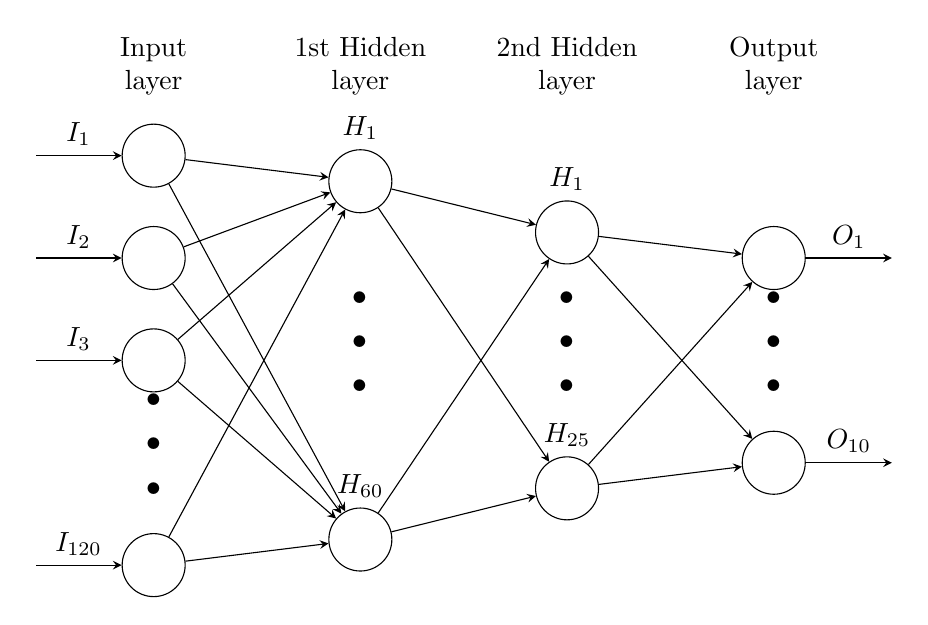
\begin{tikzpicture}[x=1.5cm, y=1.3cm, >=stealth]
        
        % layers
        \foreach \m/\l [count=\y] in {1,2,3,missing,4}
        \node [every neuron/.try, neuron \m/.try] (input-\m) at (0,2.5-\y) {};
        
        \foreach \m [count=\y] in {1,missing,2}
        \node [every neuron/.try, neuron \m/.try ] (hidden-\m) at (1.75,3-\y*1.75) {};
        
        \foreach \m [count=\y] in {1,missing,2}
        \node [every neuron/.try, neuron \m/.try ] (hidden2-\m) at (3.5,2-\y*1.25) {};
        
        \foreach \m [count=\y] in {1,missing,2}
        \node [every neuron/.try, neuron \m/.try ] (output-\m) at (5.25,1.5-\y) {};
        
        %   label
        \foreach \l [count=\i] in {1,2,3,{120}}
        \draw [<-] (input-\i) -- ++(-1,0)
        node [above, midway] {$I_{\l}$};
        
        \foreach \l [count=\i] in {1,60}
        \node [above] at (hidden-\i.north) {$H_{\l}$};
        
        \foreach \l [count=\i] in {1,25}
        \node [above] at (hidden2-\i.north) {$H_{\l}$};
        
        \foreach \l [count=\i] in {1,10}
        \draw [->] (output-\i) -- ++(1,0)
        node [above, midway] {$O_{\l}$};
        
        \foreach \i in {1,...,4}
        \foreach \j in {1,...,2}
        \draw [->] (input-\i) -- (hidden-\j);
        
        \foreach \i in {1,...,2}
        \foreach \j in {1,...,2}
        \draw [->] (hidden-\i) -- (hidden2-\j);
        
        \foreach \i in {1,...,2}
        \foreach \j in {1,...,2}
        \draw [->] (hidden2-\i) -- (output-\j);
        
        \foreach \l [count=\x from 0] in {Input, 1st Hidden, 2nd Hidden, Output}
        \node [align=center, above] at (\x*1.75,2) {\l \\ layer};
        
    \end{tikzpicture}
\end{center}

As the last dataset is the one where accuracy is the highest, this is 
also the starting point architecture for parameters optimization.

\paragraph{Activation and loss functions}
The activation function for the input and hidden layers is a \emph{Relu}, 
typically used to prevent the \emph{vanishing gradient problem}, 
and the output one uses a \emph{Softmax} to have classification probabilities
among classes.~\cite{relu}\cite{soft}\cite{vanishing}\\
The loss used is the \emph{Sparse Categorical Crossentropy loss} as it 
is well suited for multiclass classification and, since 
the classes are integers and not one-hot encoded, the sparse version is preferred.~\cite{entropy}

\paragraph{Choosing an optimizer}
When choosing an optimizer for a neural network one must take into account the 
cost of reaching a minimum point on the error function.
Although more complex optimizers exist, build to reduce training 
cost or achieve better performances on deep networks, the one choosen 
for this model is a classic Stochastic Gradient Descent optimizer.

Testing some more advanced optimizers shows that convergence is reached faster on the 
networks used in the experiments, but the speed increase is negligible as the model
is quite small.

\subsection{Initial training set results}

Section \vref{feature-extraction} talks about the four different 
training sets obtained from the dataset and, without going into details, 
states that there is continuous improvement. 
We now give a more detailed look on training performances, after 
detailing how class imbalance is faced and the applied validation method.

Note that all the random seeds used by Tensorflow are fixed 
to make results reproducible. This step is necessary as many parameters initial 
value is random, for instance, the neural network weights.

\paragraph{Class imbalance}
To deal with the minority of some classes, balancing techniques should be 
applied when fitting the model. One of the possible approaches, and the one followed
here, is to assign class weights. 

The main idea is to penalize errors made on not well represented classes to account 
for their minority. Class weights computation relies on the \emph{compute class weights} function
from sklearn.~\cite{classweight}\\
The following are the computed quantities for the dataset classes:
\begin{center}
    \begin{tabular}{ |l|c|c| } 
        \hline
        Class name & Number of samples & Class weight \\
        \hline
        air conditioner & 500 & 0.8998 \\
        car horn & 208 & 2.1629 \\
        children playing & 500 & 0.8998 \\
        dog bark & 500 & 0.8998 \\
        drilling & 500 & 0.8998 \\
        engine idling & 517 & 0.8702 \\
        gun shot & 190 & 2.3678 \\
        jackhammer & 548 & 0.8209 \\
        siren & 536 & 0.8393 \\
        street music & 500 & 0.8998 \\
        \hline
    \end{tabular}
\end{center}
As expected, the less numerous classes have higher class weight than the rest,
in particular, the misclassification of a car horn sample
counts more than double than an air conditioner one.

\paragraph{Stratified cross-validation}
To estimate performance on the training set, stratified cross-validation with 
five folds is used. Basically the dataset is divided into five parts 
and a model is repeatedly trained on four and tested on one, all while considering class 
distribution, indeed, the original distribution of the classes is maintained 
in the splits.~\cite{stratified}

The stratified approach is required as there is class imbalance on the training set.
In fact, applying a classical cross-validation could show misleading results, 
for instance when the minority classes are more present 
in the test fold rather than the training ones; in such cases the loss would be 
higher.
The mean accuracy on the test folds gives a hint about the model performance.

For this step the \emph{Stratified KFold} class from scikit learn was used.~\cite{cross-scikit}

\paragraph{Results}
For each presented training set, a model is defined 
with the structure presented at the beginning of this Section, 
and these are the results:

\begin{center}
    \begin{tabular}{ |l|r|r| } 
        \hline
        Training set & Mean accuracy & St. deviation \\
        \hline
        132 features unscaled &  0.1138 & 0.0039 \\
        132 features scaled &  0.5743 & 0.0324 \\
        144 features scaled &  0.6079 & 0.0486 \\
        120 features reduced with PCA &  0.6143 & 0.0481 \\
        \hline
    \end{tabular}
\end{center}

There is a great improvement after scaling the training set, after 
that small refinements are made.
As accuracy is the best on the last dataset, this is the one selected to 
perform the hyperparameter tuning.

\subsection{Hyperparameter tuning}

Choosing the training set with PCA applied lead to the best results 
with stratified cross-validation. Although the model is reasonable, 
it can not be the final one, as many parameters are left on their default value, 
for instance, learning rate and momentum of the optimizer are untouched. 

The main goal now is to experiments with ranges of model parameters 
to find a better one.

\paragraph{Grid and random search comparison}
Two of the most commonly used strategies in hyperparameter optimization
are \emph{grid} and \emph{random search}~\cite{random-grid}. 

In both cases we define ranges of parameters to test different combinations, 
for instance, fixed the number of neurons, one could try to find the best 
combination of learning rate and momentum that optimize accuracy on the training set.

While similar, the two methodologies differs in the amount of exploration they do.
The grid search try all the possible combinations of parameters, while the 
random approach fixes a number of iterations and picks an arbitrary combination each time. 

Obviously the first one is more computationally expensive than the second, if 
we fix a small amount of possible iterations, but in theory it finds a better result
than going the random route. 
Nonetheless the grid search can led to over-fitting and in practice random 
search in preferred.

\paragraph{Random search}
We now run a random search with various parameters 
to optimize the initial model.
Note that class weights are still considered and the models are evaluated
again with a stratified cross-validation.
The optimizer used is the stochastic gradient descent.

The considered ranges for parameters for this run are: 
\begin{enumerate}
    \item \emph{Neurons}: first and last layers stay the same, while 
    the two hidden layers are tested with a number of neurons respectively 
    equals to: 
    $$60 + 2i\;\;\text{and}\;\;25 + 2j,\;\;\text{with}\;\; i, j \in \{-2,-1,0,1,2\}$$
    \item \emph{Learning rate}: $0.001, 0.01, 0.1, 0.5$;
    \item \emph{Momentum}: $0.0, 0.01, 0.1, 1$.
\end{enumerate}

The models are fitted with 100 \emph{epochs} and \emph{batch size} equals to 32.
The two last parameters are fixed as, after various random search rounds, 
giving them a range seems to not bring any relevant 
improvement to the model found.

An early stopper is used on the training to stop it when no progress is made with 
respect to the last epoch results.
The total possible models are 400, but the search is performed with 100 iterations
in total.

\paragraph{Final model}
The best model found is the following: 
\begin{itemize}
    \item \emph{Neurons}: 120 for input, 62 for the first hidden layer, 27 for the second, and 10 for output; 
    \item \emph{Momentum}: 0.0;
    \item \emph{Learning rate}: 0.1.
\end{itemize}
Comparing the initial model with the one found now, a small improvement 
can be seen in accuracy despite a worse standard deviation:
\begin{center}
    \begin{tabular}{ |l|r|r| } 
        \hline
        Model & Mean accuracy & St. deviation \\
        \hline
        Initial model & 0.6143 & 0.0481\\
        Random search result & 0.6297 & 0.0530 \\
        \hline
    \end{tabular}
\end{center}
This network is the one chosen to evaluate performance on the test sets.
\newpage
\section{Conclusions}
\label{results}

This last Section shows the results obtained by the model found 
on the previous Section on the different test sets and
gives an overview about possible future works to be made.

\subsection{Test set results}
As stated on the first Section, the five test sets are made out of the 
folds number five, seven, eight, nine and ten.
Evaluating the model found by the Random Search on the test sets 
gives the following results: 

\begin{center}
    \begin{tabular}{ |l|r| } 
        \hline
        Test set & Accuracy\\
        \hline
        Fold 5 & 0.6496 \\
        Fold 7 & 0.6169 \\
        Fold 8 & 0.7395 \\
        Fold 9 & 0.6789 \\
        Fold 10 & 0.6774 \\ 
        \hline
    \end{tabular}
\end{center}

Finally, the mean accuracy and standard deviation are: 
\begin{center}
    \begin{tabular}{ |r|r| } 
        \hline
        Mean accuracy & Standard deviation\\
        \hline
        0.6724 & 0.0403 \\
        \hline
    \end{tabular}
\end{center}

\subsection{Future works}

The results on the test sets are promising, but there is definitely 
room for improvement.

Indeed, a more refined training set creation can be made, by exploiting 
more features from the Librosa library, testing different type 
of scalers and experimenting with different feature selection 
techniques.

Finally, the models used in the project are simple, more complex 
Neural Networks, for instance with Convolutional layers, could 
perform better, also, a more extensive random search might improve
results.

\newpage

\addcontentsline{toc}{section}{References}
\bibliography{chapters/bibliography}
\bibliographystyle{unsrt}

\end{document}